% tikz_radii.tex -- fig:radii, the radii that decide which centres can cut V_c.
%   A plane through the centre c = 0, to scale.  The half-space of a centre y
%   is <x, y/|y|> <= |y|/2.  A contact (|y| = 2) is tangent to the unit ball;
%   a centre at distance d in (2, sqrt6) cuts a cap off B(sqrt(3/2)), whose
%   half-chord is sqrt(3/2 - d^2/4) (0.484 at d = 2.25); at d = sqrt6 the
%   bisector is tangent to B(sqrt(3/2)); at d = 2 sqrt2 it is tangent to
%   B(sqrt2), the circumscribed ball of the 24-cell.
% Test:   python3 tikz_overlap_check.py tikz_radii.tex
% Build:  pdflatex tikz_radii.tex && pdftoppm -r 500 -png -singlefile tikz_radii.pdf ../figures/fig_tikz_radii
\documentclass[border=4pt]{standalone}
\usepackage{tikz}
\usetikzlibrary{calc,arrows.meta}
\usepackage[T1]{fontenc}
\usepackage{lmodern}
\usepackage{amsmath,amssymb}
\definecolor{cblue}{HTML}{2A78D6}
\definecolor{corange}{HTML}{EB6834}
\definecolor{caqua}{HTML}{1BAF7A}
\definecolor{cink}{HTML}{0B0B0B}
\definecolor{cink2}{HTML}{52514E}
\definecolor{cink3}{HTML}{8B8A85}
\definecolor{cpanel}{HTML}{F4F3EF}
% tikzcheck.tex -- the hooks of tikz_overlap_check.py, input by the TikZ figures.
% Two ways to name what is checked.
%  - Explicit: \figboxes and \figlabels list named nodes; with \nolabels defined,
%    nodes in the style lbl are drawn invisibly.
%  - Automatic: \autocheck in the preamble gives every node of the picture,
%    pgfplots tick labels included, an alias chk<n>; with \nolabels defined, the
%    text of every node is drawn invisibly and its shape is kept.
% \checkfigure, at the end of the picture, writes the four corners of each
% checked node (so that rotated nodes are measured by their true extent) and
% those of the picture to the log when \checkbboxes is defined.
\tikzset{lbl/.style={}}
\ifdefined\nolabels\tikzset{lbl/.append style={opacity=0}}\fi
\newcount\chknodes
\newcommand\autocheck{% idempotent: a figure with \autocheck may also be run with --auto
  \ifdefined\chkauto\else
  \def\chkauto{}%
  \tikzset{every node/.append style={/utils/exec={\global\advance\chknodes by 1\relax},
                                      alias=chk\the\chknodes}}%
  \ifdefined\nolabels\tikzset{every node/.append style={text opacity=0}}\fi
  \fi}
\makeatletter
% a node counted but never kept (pgfplots typesets some nodes once to measure them)
% has no shape, and is skipped
\newcommand\chkifnode[2]{\pgfutil@ifundefined{pgf@sh@ns@#1}{}{#2}}
\makeatother
\newcommand\chkout[2]{% kind, node
  \path let \p1=(#2.south west), \p2=(#2.north east), \p3=(#2.north west), \p4=(#2.south east)
    in \pgfextra{\typeout{BBOX #1 #2\space\x1\space\y1\space\x2\space\y2\space\x3\space\y3\space\x4\space\y4}};}
\newcommand\checkfigure{%
  \ifdefined\checkbboxes
    \path let \p1=(current bounding box.south west), \p2=(current bounding box.north east)
      in \pgfextra{\typeout{PICBB \x1\space\y1\space\x2\space\y2}};
    \typeout{BORDER 4.0pt}%
    \ifdefined\chkauto
      \edef\chklast{\the\chknodes}%
      \foreach \nm in {1,...,\chklast} {\chkifnode{chk\nm}{\chkout{auto}{chk\nm}}}%
    \else
      \foreach \nm in \figboxes {\chkout{box}{\nm}}%
      \foreach \nm in \figlabels {\chkout{label}{\nm}}%
    \fi
  \fi}
\ifdefined\forceauto\autocheck\fi

\autocheck
\begin{document}
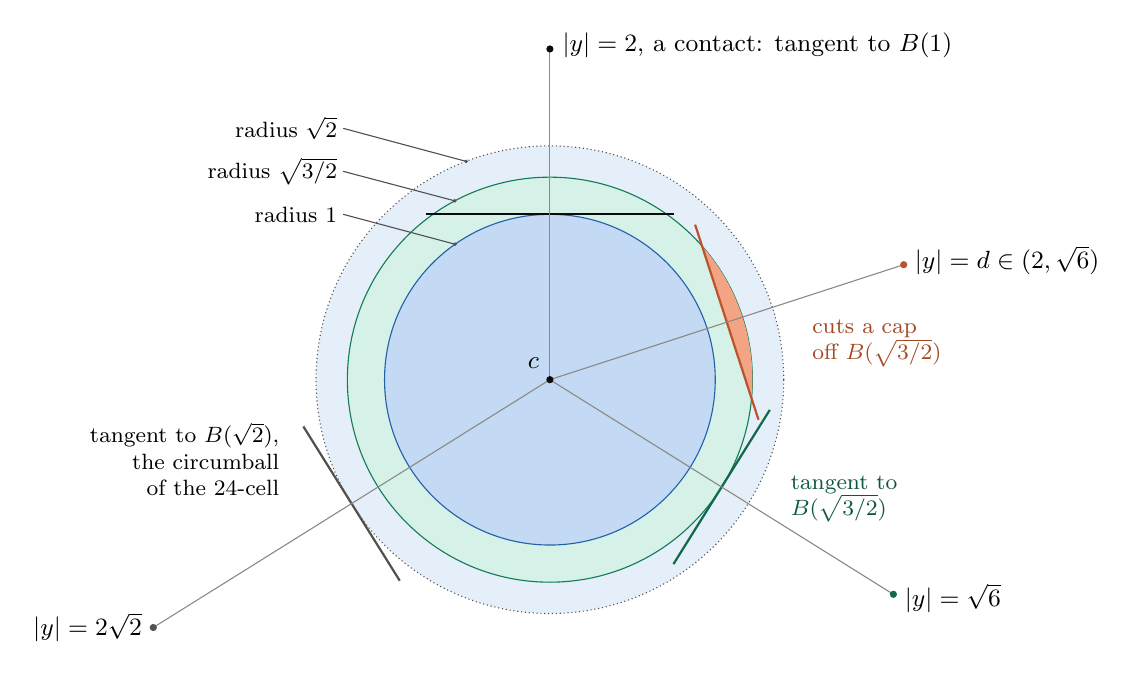
\begin{tikzpicture}[font=\small, x=2.1cm, y=2.1cm]
  % balls about c
  \fill[cblue!12] (0,0) circle (1.41421);
  \fill[caqua!18] (0,0) circle (1.22474);
  \fill[cblue!28] (0,0) circle (1);
  \draw[cink2, densely dotted] (0,0) circle (1.41421);
  \draw[caqua!70!black, thin] (0,0) circle (1.22474);
  \draw[cblue!80!black, thin] (0,0) circle (1);
  % cap of the centre at distance 2.25, direction 18 deg
  \begin{scope}[rotate=18]
    \clip (0,0) circle (1.22474);
    \fill[corange!60] (1.125,-0.6) rectangle (1.4,0.6);
  \end{scope}
  % bisectors
  \draw[cink, thick] (-0.75,1) -- (0.75,1);                                  % contact, |y| = 2
  \draw[corange!80!black, thick, rotate=18] (1.125,-0.62) -- (1.125,0.62);  % |y| = 2.25
  \draw[caqua!60!black, thick, rotate=-32] (1.22474,-0.55) -- (1.22474,0.55); % |y| = sqrt6
  \draw[cink2, thick, rotate=212] (1.41421,-0.55) -- (1.41421,0.55);         % |y| = 2 sqrt2
  % centres and rays
  \foreach \p in {(0,2), (2.1399,0.6953), (2.0773,-1.2980), (-2.3986,-1.4988)}
    \draw[cink3, thin] (0,0) -- \p;
  \fill[cink] (0,0) circle (1.3pt);
  \fill[cink] (0,2) circle (1.3pt);
  \fill[corange!80!black] (2.1399,0.6953) circle (1.3pt);
  \fill[caqua!60!black] (2.0773,-1.2980) circle (1.3pt);
  \fill[cink2] (-2.3986,-1.4988) circle (1.3pt);
  % labels of the centres
  \node[anchor=west, inner sep=2pt] at (0.04,2.02) {$|y|=2$, a contact: tangent to $B(1)$};
  \node[anchor=west, inner sep=2pt] at (2.17,0.72) {$|y|=d\in(2,\sqrt6)$};
  \node[anchor=west, inner sep=2pt] at (2.11,-1.32) {$|y|=\sqrt6$};
  \node[anchor=east, inner sep=2pt] at (-2.43,-1.50) {$|y|=2\sqrt2$};
  \node[anchor=south east, inner sep=2pt] at (-0.03,0.03) {$c$};
  % radii, with leaders
  \fill[cink2] (125:1) circle (0.7pt);
  \fill[cink2] (118:1.22474) circle (0.7pt);
  \fill[cink2] (111:1.41421) circle (0.7pt);
  \draw[cink2, thin] (125:1) -- (-1.25,1.0);
  \draw[cink2, thin] (118:1.22474) -- (-1.25,1.26);
  \draw[cink2, thin] (111:1.41421) -- (-1.25,1.52);
  \node[anchor=east, inner sep=2pt, font=\footnotesize] at (-1.25,1.0) {radius $1$};
  \node[anchor=east, inner sep=2pt, font=\footnotesize] at (-1.25,1.26) {radius $\sqrt{3/2}$};
  \node[anchor=east, inner sep=2pt, font=\footnotesize] at (-1.25,1.52) {radius $\sqrt2$};
  % what each bisector does
  \node[anchor=west, inner sep=2pt, font=\footnotesize, text=corange!70!black, align=left] at (1.55,0.22) {cuts a cap\\ off $B(\sqrt{3/2})$};
  \node[anchor=west, inner sep=2pt, font=\footnotesize, text=caqua!50!black, align=left] at (1.42,-0.72) {tangent to\\ $B(\sqrt{3/2})$};
  \node[anchor=east, inner sep=2pt, font=\footnotesize, align=right] at (-1.6,-0.48) {tangent to $B(\sqrt2)$,\\ the circumball\\ of the $24$-cell};
\checkfigure
\end{tikzpicture}
\end{document}
